\subsection{UC11 - Visualizzazione del menu' ristorante} \label{usecase:11}
\begin{figure}[H]
    \centering
    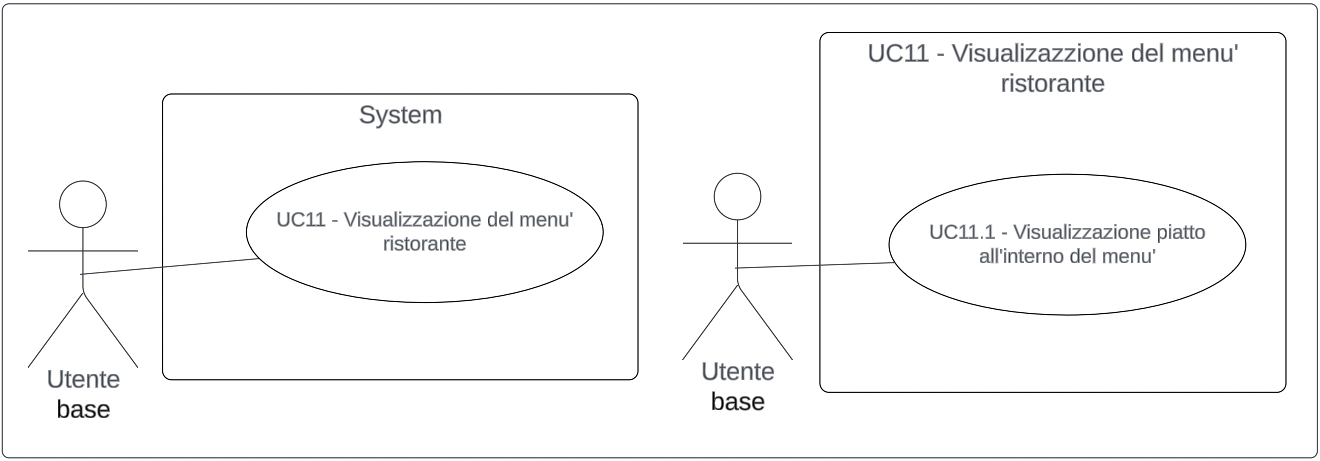
\includegraphics[width=0.9\linewidth]{ucd/UCD11_new.png}
\caption{Visualizzazione del menu' ristorante}
\end{figure}
\textbf{Attori}:
\begin{itemize}
    \item Utente base.
\end{itemize}
\textbf{Precondizioni}:
\begin{itemize}
    \item L'utente ha scelto il menu' di un ristorante da visualizzare.
\end{itemize}
\textbf{Postcondizioni}:
\begin{itemize}
    \item L'utente ha visualizzato il menu' del ristorante.
\end{itemize}
\textbf{Scenario principale}:
\begin{enumerate}
    \item L'utente visualizza la lista dei piatti presenti nel menu';
    \item L’utente visualizza il piatto con relativo nome, prezzo e lista di ingredienti (\nameref{usecase:11_1}).
\end{enumerate}
\begin{comment}
% Forse non ci va perche non è un errore se la lista è vuota(?)
\textbf{Scenari alternativi}: % o secondari
\begin{enumerate}
    \item Il menu' è vuoto (non sono presenti piatti inseriti dall'amministratore oppure i criteri di ricerca non restituiscono piatti corrispondenti) e viene visualizzato un messaggio di errore
\end{enumerate}
\end{comment}